\chapter{Simulations}
This Chapter show the simulation results of our 5G PDSCH simulator, before getting into the results and performance of our simulator, let's see our simulation parameters.
\section{Channel Parameters}
As mentioned before, our system is OFDM based using a block fading channel.
\begin{GrayBox}
    \textbf{Note:} Our performance metric of interest are the BER \& BLER.
\end{GrayBox}
The shown graphs in this chapter depicts relationship of (BER and BLER) vs $E_b$/$No$ for various setups of our simulator.\\
The simulation parameters per $E_b$/$No$ is shown in Table~\ref{tbl:ch parameters}.
\begin{table}[H]
    \centering
    \caption{Simulation Parameters per $E_b$/$N_o$}
    \label{tbl:ch parameters}
    \begin{tabular}{ll}
        \toprule
        Parameter & Value \\
        \midrule
        \# of Frames & 100 \\
        Slots per Frame & 100 (For Linear Coding) \\
                        & 50 (For LDPC Coding) \\
        OFDM Symbols per Slot & 14 \\
        \# of Sub-carriers per OFDM Symbol & 1024 \\
        Modulation Order & BPSK \\
                         & QPSK \\
                         & 16 QAM \\
                         & 64 QAM \\
                         & 265 QAM \\
        Input/Output Setup & SISO \\
                           & SIMO \\
                           & MISO \\
                           & MIMO (Diversity) \\
                           & MIMO (Spatial Multiplexing) \\
        Channel Coding & Linear Block Code with Coding Rate = $\frac{4}{7}$ \\
                       & LDPC with Coding Rate = $\frac{4}{7}$ \\
        Channel Variance & 0.03 \\
        \# of Sub-carriers in a Resource Block (RB) & 16 \\
        Coherence Time & 4 Slots \\
        Coherence Bandwidth & 4 RBs \\ 
        \# of Pilots per Channel Block & 1 (for SISO, SIMO \& MISO) \\
        & M (For MIMO) \\
        \bottomrule
    \end{tabular}
\end{table}

Other facts about reference signals and channel estimation in the system are:
\begin{itemize}
    \item CSI-RS is sent in the first OFDM symbol.
    \item DMRS is sent in the second OFDM symbol.
    \item Perfect \emph{channel feedback} from the Rx to the Tx is assumed.
    \item Resource blocks are different from 5G (which has the RB = 12 sub-carriers with 3300 sub-carriers OFDM symbol) just for simplicity.
    \item For all MIMO setups, number of pilots per channel block can range up to 64 pilots which are used to get more than channel estimate for each channel block and get the average estimation.
\end{itemize}

\section{Results}
Here we take a look at the results of the simulation in the following cases:
\begin{itemize}
    \item 16 QAM SISO linear vs ldpc with rate = $4/7$
    \item BPSK SISO linear, channel variance = $0.03$ vs $1$
    \item LDPC rate $4/7$ SIMO $1 \times 2$ (all modulation orders: BPSK, QPSK, 16 QAM \& 64 QAM)
    \item BPSK SISO LDPC rate = $1/3$ vs $4/7$
\end{itemize}

\subsection{16 QAM SISO: Linear vs LDPC with rate = $4/7$}
\subsubsection{BER}
\begin{figure}[H]
    \centering
    \includegraphics[width=.75\textwidth]{Results/1/BER.png}
    \caption{16 QAM SISO BER: Linear vs LDPC with rate = 4/7}
\end{figure}
\subsubsection{BLER}
\begin{figure}[H]
    \centering
    \includegraphics[width=.75\textwidth]{Results/1/BLER.png}
    \caption{16 QAM SISO BLER: Linear vs LDPC with rate = 4/7}
\end{figure}

\subsection{BPSK SISO Linear: channel variance = $0.03$ vs $1$}
\subsubsection{BER}
\begin{figure}[H]
    \centering
    \includegraphics[width=.75\textwidth]{Results/2/BER.png}
    \caption{BPSK SISO Linear BER: channel variance = 0.03 vs 1}
\end{figure}
\subsubsection{BLER}
\begin{figure}[H]
    \centering
    \includegraphics[width=.75\textwidth]{Results/2/BLER.png}
    \caption{BPSK SISO Linear BLER: channel variance = 0.03 vs 1}
\end{figure}

\subsection{LDPC rate $4/7$ SIMO $1 \times 2$ (all modulation orders: BPSK, QPSK, 16 QAM \& 64 QAM)}
\subsubsection{BER}
\begin{figure}[H]
    \centering
    \includegraphics[width=.75\textwidth]{Results/3/BER.png}
    \caption{BER: LDPC rate 4/7 SIMO 1 x 2 (all modulation orders: BPSK, QPSK, 16 QAM \& 64 QAM)}
\end{figure}
\subsubsection{BLER}
\begin{figure}[H]
    \centering
    \includegraphics[width=.75\textwidth]{Results/3/BLER.png}
    \caption{BLER: LDPC rate 4/7 SIMO 1 x 2 (all modulation orders: BPSK, QPSK, 16 QAM \& 64 QAM)}
\end{figure}

\subsection{BPSK SISO LDPC rate = $1/3$ vs $4/7$}
\subsubsection{BER}
\begin{figure}[H]
    \centering
    \includegraphics[width=.75\textwidth]{Results/4/BER.png}
    \caption{BPSK SISO BER: LDPC rate = 1/3 vs 4/7}
\end{figure}
\subsubsection{BLER}
\begin{figure}[H]
    \centering
    \includegraphics[width=.75\textwidth]{Results/4/BLER.png}
    \caption{BPSK SISO BLER: LDPC rate = 1/3 vs 4/7}
\end{figure}